\documentclass{article}
%------------------------------------PACKAGES
\usepackage[utf8]{inputenc}
\usepackage{graphicx}
\usepackage{setspace}
\usepackage{listings}
\usepackage{xcolor}
\usepackage{amsmath}

\title{Merge sort}
\author{Amirhosein Noroozi}
\date{December 2020}

\begin{document}

\maketitle

\section{Introduction}

{In computer science, merge sort (also commonly spelled mergesort) is an efficient, general-purpose, comparison-based sorting algorithm. Most implementations produce a stable sort, which means that the order of equal elements is the same in the input and output. Merge sort is a divide and conquer algorithm that was invented by John von Neumann in 1945.[2] A detailed description and analysis of bottom-up merge sort appeared in a report by Goldstine and von Neumann as early as 1948.}
\section{Algorithm}
  Conceptually, a merge sort works as follows:

    1.Divide the unsorted list into n sublists, each containing one element (a list of one element is considered sorted).

2.Repeatedly merge sublists to produce new sorted sublists until there is only one sublist remaining. This will be the sorted list.
\newpage
\section{Example}
\begin{figure}[h!]
\centering
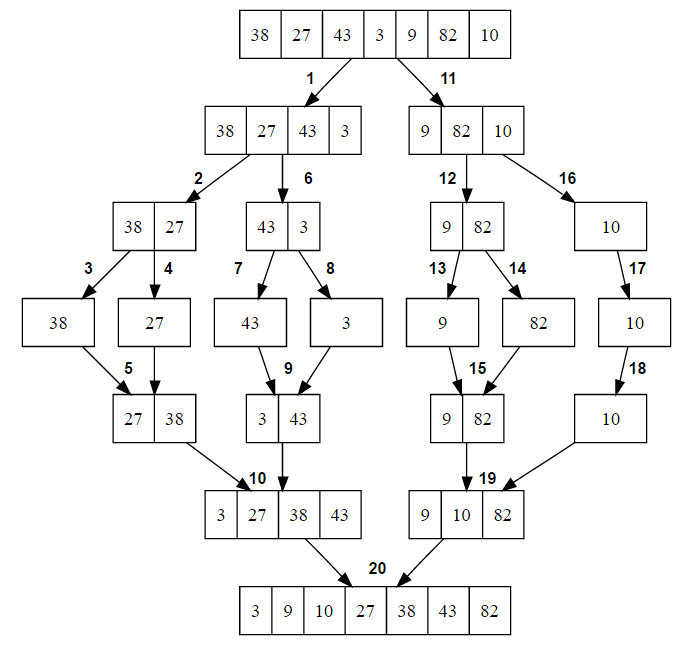
\includegraphics[scale=0.7]{MergeSort.jpg}
\caption{MergeSort}
\label{fig:MergeSort}
\end{figure}
\newpage
\section{Natural merge sort}
A natural merge sort is similar to a bottom-up merge sort except that any naturally occurring runs (sorted sequences) in the input are exploited. Both monotonic and bitonic (alternating up/down) runs may be exploited, with lists (or equivalently tapes or files) being convenient data structures (used as FIFO queues or LIFO stacks).[4] In the bottom-up merge sort, the starting point assumes each run is one item long. In practice, random input data will have many short runs that just happen to be sorted. In the typical case, the natural merge sort may not need as many passes because there are fewer runs to merge. In the best case, the input is already sorted (i.e., is one run), so the natural merge sort need only make one pass through the data. In many practical cases, long natural runs are present, and for that reason natural merge sort is exploited as the key component of Timsort. Example:
\begin{table}[h]
    \begin{center}
         \begin{tabular}{|c|c|}
            \hline
            Start & 3  4  2  1  7  5  8  9  0  6\\
            \hline
            Select runs & (3  4)(2)(1  7)(5  8  9)(0  6)\\
            \hline
            Merge & (2  3  4)(1  5  7  8  9)(0  6)\\
            \hline
            Merge & (1  2  3  4  5  7  8  9)(0  6)\\
            \hline
            Merge & (0  1  2  3  4  5  6  7  8  9)\\
            \hline
        \end{tabular}
    \end{center}
\end{table}

Tournament replacement selection sorts are used to gather the initial runs for external sorting algorithms.

\newpage
\section{Analysis}
In sorting n objects, merge sort has an average and worst-case performance of O(n log n). If the running time of merge sort for a list of length n is T(n), then the recurrence relation T(n) = 2T(n/2) + n follows from the definition of the algorithm (apply the algorithm to two lists of half the size of the original list, and add the n steps taken to merge the resulting two lists). The closed form follows from the master theorem for divide-and-conquer recurrences.

The number of comparisons made by merge sort in the worst case is given by the sorting numbers. These numbers are equal to or slightly smaller than$ (n  {\lceil} lg n{\rceil}  - 2 ^ {{\lceil} lg n{\rceil}}  + 1)$, which is between $ (n lg n - n + 1) $ and $(n lg n + n + O(lg n))$. Merge sort's best case takes about half as many iterations as its worst case.

For large n and a randomly ordered input list, merge sort's expected (average) number of comparisons approaches ${\alpha} {\cdot} n$ fewer than the worst case, where

${\displaystyle {\alpha} =-1+\sum _{k=0}^{\infty }{\frac {1}{2^{k}+1}}\approx 0.2645.}$

In the worst case, merge sort uses approximately 39\% fewer comparisons than quicksort does in its average case, and in terms of moves, merge sort's worst case complexity is O(n log n) - the same complexity as quicksort's best case.

Merge sort is more efficient than quicksort for some types of lists if the data to be sorted can only be efficiently accessed sequentially, and is thus popular in languages such as Lisp, where sequentially accessed data structures are very common. Unlike some (efficient) implementations of quicksort, merge sort is a stable sort.

Merge sort's most common implementation does not sort in place; therefore, the memory size of the input must be allocated for the sorted output to be stored in (see below for variations that need only n/2 extra spaces).
%-------------------------------------CODE
\newpage
\section{Code}
\begin{lstlisting}[language=C++]
    // C++ program for Merge Sort
    #include <iostream>
    using namespace std;
    
    // Merges two subarrays of arr[].
    // First subarray is arr[l..m]
    // Second subarray is arr[m+1..r]
    void merge(int arr[], int l, int m, int r)
    {
    	int n1 = m - l + 1;
    	int n2 = r - m;
    
    	// Create temp arrays
    	int L[n1], R[n2];
    
    	// Copy data to temp arrays L[] and R[]
    	for (int i = 0; i < n1; i++)
    		L[i] = arr[l + i];
    	for (int j = 0; j < n2; j++)
    		R[j] = arr[m + 1 + j];
    
    	// Merge the temp arrays back into arr[l..r]
    
    	// Initial index of first subarray
    	int i = 0;
    
    	// Initial index of second subarray
    	int j = 0;
    
    	// Initial index of merged subarray
    	int k = l;
    
    	while (i < n1 && j < n2) {
    		if (L[i] <= R[j]) {
    			arr[k] = L[i];
    			i++;
    		}
    		else {
    			arr[k] = R[j];
    			j++;
    		}
    		k++;
    	}
    
    	// Copy the remaining elements of
    	// L[], if there are any
    	while (i < n1) {
    		arr[k] = L[i];
    		i++;
    		k++;
    	}
    
    	// Copy the remaining elements of
    	// R[], if there are any
    	while (j < n2) {
    		arr[k] = R[j];
    		j++;
    		k++;
    	}
    }
    
    // l is for left index and r is
    // right index of the sub-array
    // of arr to be sorted */
    void mergeSort(int arr[],int l,int r){
    	if(l>=r){
    		return;//returns recursively
    	}
    	int m = (l+r-1)/2;
    	mergeSort(arr,l,m);
    	mergeSort(arr,m+1,r);
    	merge(arr,l,m,r);
    }
    
    // UTILITY FUNCTIONS
    // Function to print an array
    void printArray(int A[], int size)
    {
    	for (int i = 0; i < size; i++)
    		cout << A[i] << " ";
    }
    
    // Driver code
    int main()
    {
    	int arr[] = { 12, 11, 13, 5, 6, 7 };
    	int arr_size = sizeof(arr) / sizeof(arr[0]);
    
    	cout << "Given array is \n";
    	printArray(arr, arr_size);
    
    	mergeSort(arr, 0, arr_size - 1);
    
    	cout << "\nSorted array is \n";
    	printArray(arr, arr_size);
    	return 0;
    }
\end{lstlisting}

\end{document}
